\section{Accumulation of Special Parameter Values on Homoclinic Parameter Values}\label{hcs}
			In this section we will discuss the interesting behavior as the system admits a homoclinic point as defined below.

			\begin{mydef}{Local Unstable Set\cite{Dev2}}
			Let $f (p) = p, \ |f' (p)| > 1$ such that $p$ is a repelling fixed point. Then there must be an open interval about $p$ on which $f$ is one-to-one and satisfies the the expansion property $|f (x) - p| > |x - p|$. We define the local unstable set at $p$ to be the maximal such open interval about $p$. We denote this set by $W^u_{loc} (p)$.
			\end{mydef}

			\begin{mydef}{Homoclinic Point\cite{Dev2}}
			Let $f (p) = p$ and $f' (p) > 1$. A point $q$ is called homoclinic to $p$ if $q \in W^u_{loc} (p)$ and there exists $n > 0$ such that $f^n (q) = p$. The point $q$ is heteroclinic if $q \in W^u_{loc} (p)$ and there exists $n > 0$ such that $f^n (q)$ lies on a different periodic orbit
			\end{mydef}

			The Figure \ref{hc} shows a parameter value for which the critical point is homoclinic to the right hand fixed point (depicted under graphical iteration). A more intuitive way of thinking about homoclinic points is that if a point $q$ is homoclinic to $p$ then $q$ approaches $p$ under forward and backward iteration.
			\begin{figure}[h]
				\centering
				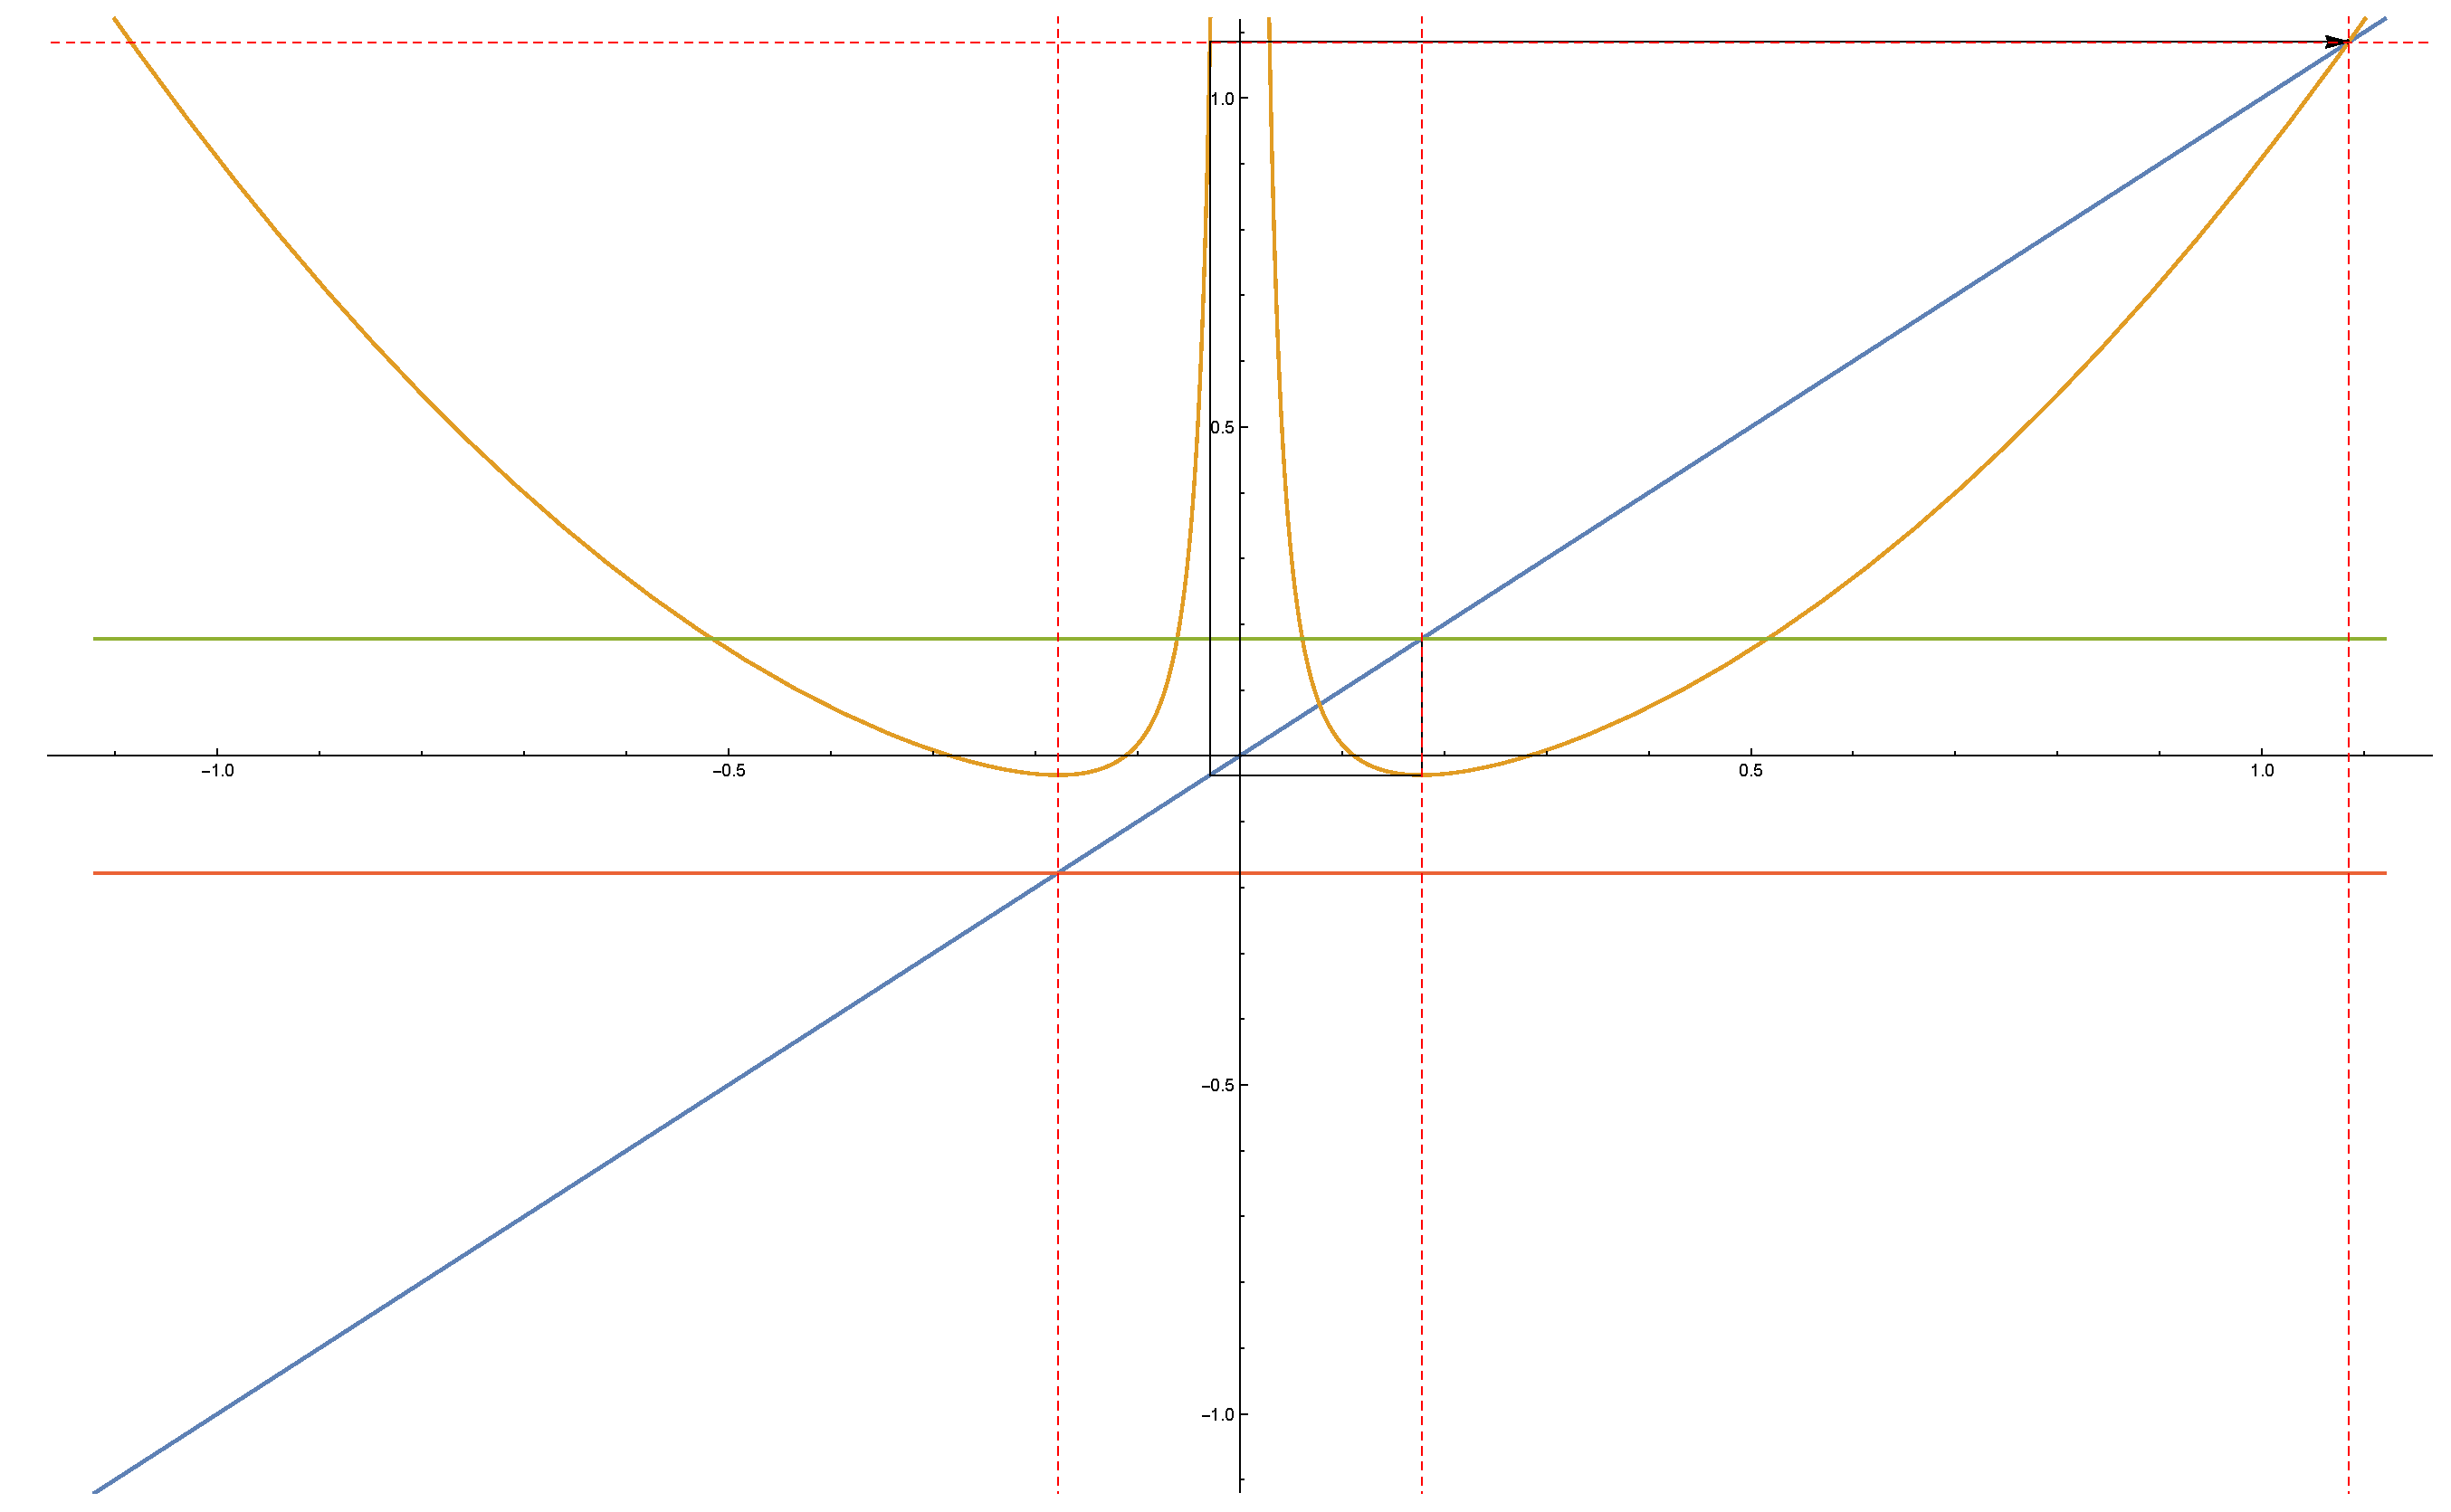
\includegraphics[width=.75\columnwidth]{./img/homoclinic.pdf}%
				\caption{Graphical iteration showing the ``primary'' homoclinic point of $f$ at the parameter value $\pr \approx -0.092395$}
				\label{hc}%
			\end{figure}
			% Another, more intuitive way of thinking about homoclinic points is that they are attracting under both forward and backward iteration. While the original quadratic map only had one such homoclinic point (CITATION/PROOF?), the singularity in our perturbed map introduces many more opportunities for homoclinic behavior, as the following proof shows:

			% \begin{myprop}
			% Every pre-zero point of order $n > 2$ admits at least one point homoclinic to the right hand fixed point $P_c$ on the interval $ (\pl, \pr)$.
			% \end{myprop}

			% \begin{myproof}
			% 	Lemma \ref{fppos} guarantees that $P_c > 0$ for all $c$. Then from Corollary \ref{maincor}, it is clear that there must exist some $c_1, c_2 \in \inte{c_1}{c_2}$ such that $f^{n}_{c_1} (C) = 0$ and $f^n_{c_2} = \infty$. Thus on the interval $\inte{c_1}{c_2}$, there must exist a $c_3$ such that $f^n_{c_3} (C) = P_c$. Thus we are prefixed at $P_c$ in forward time. Additionally since $P_c$ is cleary reprelling on this interval, the backward orbit $O^- (C)$ also approaches $P_c$. Therefore the forward and backward orbits are both approaching $P_c$ so our map $f_c$ admits a homoclinic point at the parameter value $c_3$.
			% \end{myproof}

			One requirement common to most of the subsequent arguments is that we are working with a continuous map, something that $f_c$ currently is not, given the discontinuity at zero. The following propositions allay these concerns by shifting our system to the two-point compactification of the reals, over which $f_c (x)$ is continuous. 

			\begin{myprop}\label{contin}
				The family of maps $f_c (x) = x^2 + c + \frac{.001}{x^2}$ is continuous with respect to $x$ and $c$ under the two point compactification of the reals.
			\end{myprop}

			\begin{myproof}
				Consider $f: \R \ra \R$ such that $f (x) = x^2 + c + \frac{.001}{x^2}$. Now let $\widetilde{\R} = \R \cup \{-\infty, \infty\}$ and consider $\widetilde{f}$ such that $\widetilde{f}:\widetilde{\R} \ra \widetilde{\R}$ where $f$ and $\widetilde{f}$ are equal at all points equal except $\widetilde{f} (-\infty) = \infty$, $\widetilde{f} (0) = \infty$, and $\widetilde{f} (\infty) = \infty$. Additionally consider the map $h (x) = \left (\frac{2}{\pi}\right)\arctan (x)$ where $h : \R \ra (-1,1)$ and the map $\widetilde{h} : \widetilde{\R} \ra [-1,1]$ where $h$ and $\widetilde{h}$ are at all points equal except $\widetilde{h} (-\infty) = -1$ and $\widetilde{h} (\infty) = 1$. Now consider the following conjugacy where $\widetilde{g_c} = \widetilde{h}\circ\widetilde{f_c}\circ \widetilde{h}^{-1}$:

				\begin{displaymath}
					\xymatrix
					{
						\widetilde{\R} \ar@{->}[r]^{\widetilde{f_c}}\ar@{->}[d]_{\widetilde{h}} & \widetilde{\R} \ar@{->}[d]^{\widetilde{h}}\\
						[-1,1] \ar@{->}[r]^{\widetilde{g_c}} & [-1,1]
					}
				\end{displaymath}

				Plotting $\widetilde{g_c}$ we get the image in Figure \ref{compact}. We can see that the function $\widetilde{g_c} (x)$ is clearly continuous in this extended space so we can conclude that $\widetilde{f_c} (x)$ is conjugate to a continuous map on the interval $[-1,1]$ and consequently is itself continuous.

				\begin{figure}[h]
					\centering
						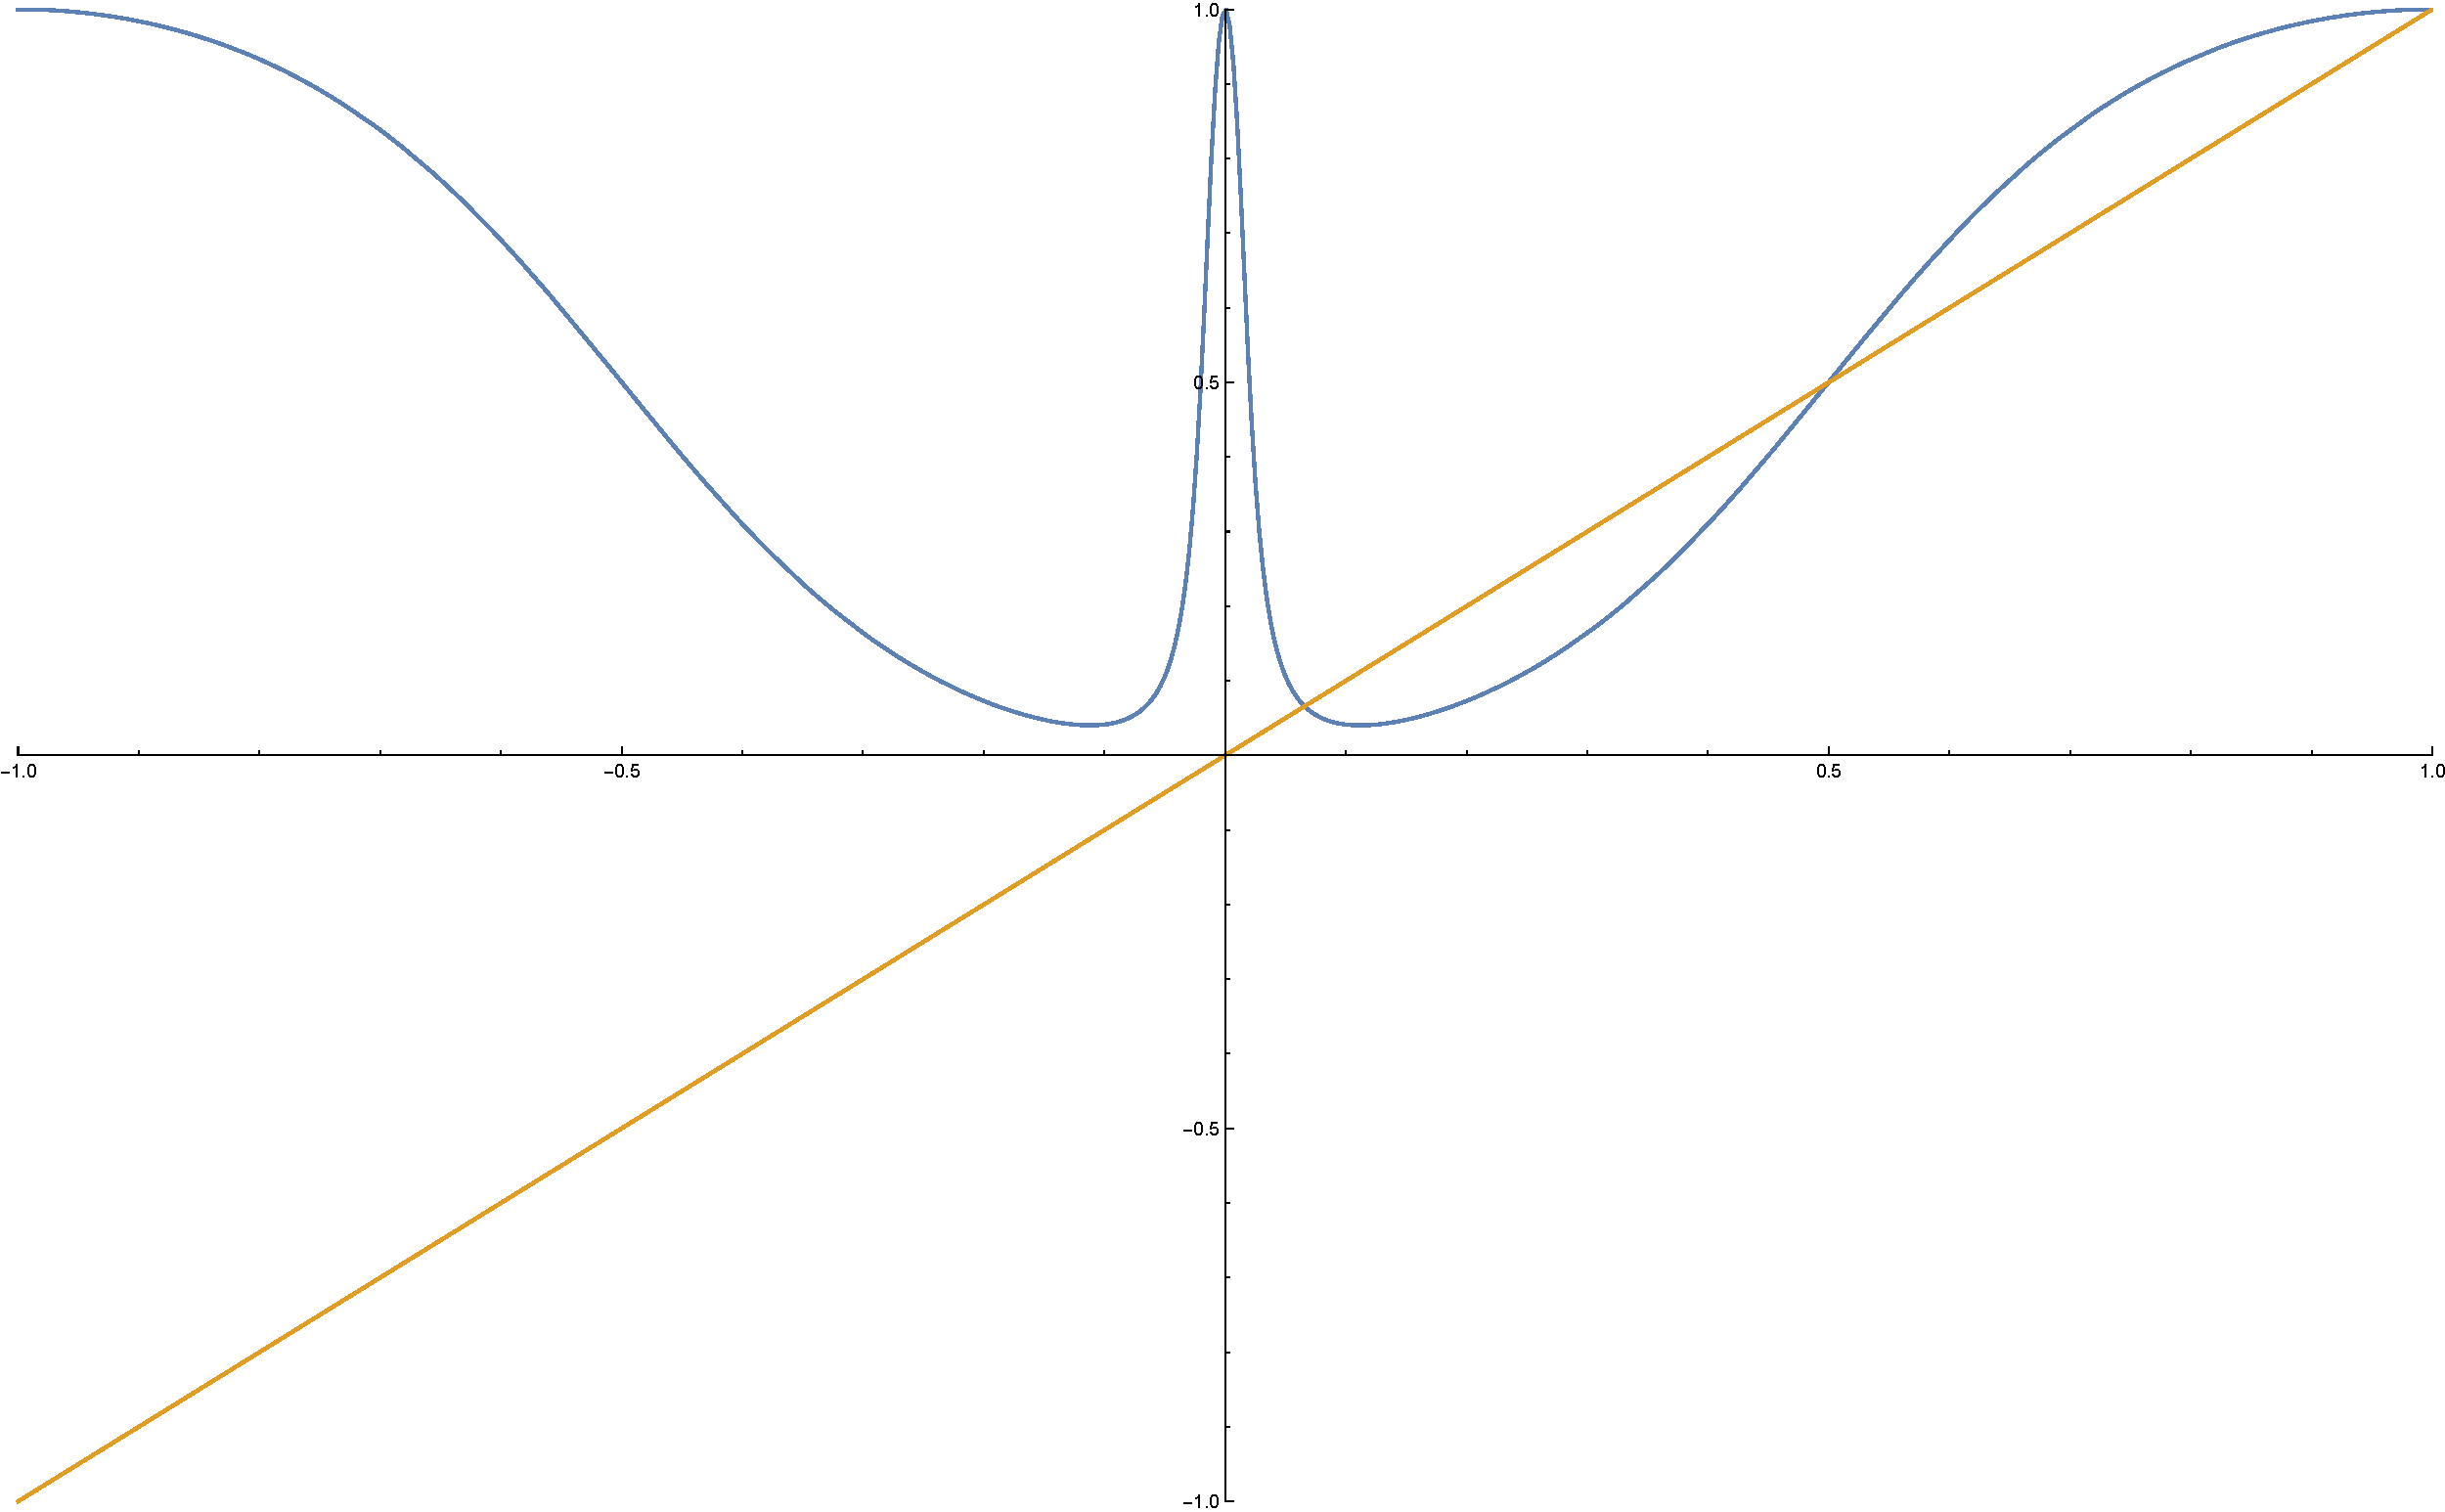
\includegraphics[width=.8\textwidth]{./img/compact.pdf}
						\caption{The continuous function $\widetilde{g_c}: [-1,1] \ra [-1,1]$ for $c = 0$ along with the reference line $y = x$}
						\label{compact}
				\end{figure}
				% Thus the only difference between $f$ and $\widetilde{f}$ is that we add points at $-\infty$ and $\infty$ such that $\widetilde{f} (-\infty) = \infty$, $f (0) = \infty$, and $f (\infty) = \infty$. To see that $\widetilde{f}$ is continuous, we first note that $f$ is continuous at all points except 0, meaning that $\widetilde{f}$ is also continuous at $\R \setminus \{0\}$. Then in order to show that $\widetilde{f}$ is continuous at 0, we simply consider the left and right limits of 0:
				% \[
				% 	\lim_{x\ra 0^-} \widetilde{f} (x) = \infty = \lim_{x \ra 0^+} \widetilde{f} (x) \text{ where }\infty \in \R \cup \{-\infty, \infty\}
				% \]
				% Thus the limit in either direction is the point $\infty$ which is now in the image of $\widetilde{f}$, so we can conclude that the function $\widetilde{f}$ is continuous with respect to $x$ for all $x$ when $c = 0$. To see that the function is also continuous with respect to $x$ for any $c$, we first note that changes in the term $c$ simply translate the curve $\widetilde{f}_c (x)$ up and down such that the points we discussed earlier are mapped in an identical way: $\widetilde{f}_c (-\infty) = \widetilde{f}_c (0) = \widetilde{f}_c (\infty) = \infty$. Therefore the argument above can be applied for any $c$ so we conclude that $\widetilde{f}_c (x) : \widetilde{\R} \ra \widetilde{\R}$ is continuous with respect to $x$ for all $x, c \in \widetilde{\R}.$
			\end{myproof}

			Thus in our extended space, we no longer need to worry about the discontinuity at 0. \textbf{For the remainder of the chapter, relabel $\widetilde{f}$ as $f$ such that $f: \widetilde{\R} \ra \widetilde{\R}$}. Additionally, we know that the composition of continuous maps is continuous so for all $n$, $f^n_c (x)$ is continuous with respect to $x$ and $c$. 

			Before proceeding further, we must develop a description of how higher iterates change with respect to $x$ and $c$. First note that 
			\al{
				\frac{\partial f_c (x)}{\partial x} &= \frac{\partial}{\partial x}\left (x^2 + c + \frac{.001}{x^2}\right) = 2x - \frac{.002}{x^3}\\
				\frac{\partial f_c (x)}{\partial c} &= \frac{\partial}{\partial c}\left (x^2 + c + \frac{.001}{x^2}\right) = 1\\
			}
			For simplicity, we will denote the first function as $f' (x) = 2x - \frac{.002}{x^3}$. Note that since $f' (x)$ has an odd degree polynomial singularity, we do not have a continuous derivative under the aforementioned compactification. Now that we have obtained our derivative with respect to $x$ and $c$, we can easily expand this to the derivative of the $n^{th}$ iterate of $f_c (x)$ by using the chain rule. For now we rewrite our function such that $f_c (x) = f (x,c)$ where we are iterating under the following function composition:
			\[
				f^n (x,c) = f^{n-1} (f (x,c),x) = f^{n-2} (f (f (x,c),c),c) = \cdots = \underbrace{f (f (f (\cdots,c),c),c)}_{n - 1 \text{ times}}
			\]
			Now let $z = f^n (x,c) = f\left (f^{n-1} (x,c),c\right) = f (v, c)$ where $v = f^{n-1} (x,c)$. Then we see that the derivative of the $n^{th}$ iterate with respect to $x$ is given by:
			\al{
				\frac{\partial z}{\partial x} &= \frac{\partial z}{\partial v} \frac{\partial v}{\partial x} + \frac{\partial z}{\partial c} \frac{\partial c}{\partial x}\\
				&=\left (\frac{\partial}{\partial v} \left (v^2 + c + \frac{.001}{v^2}\right)\right)\frac{\partial f^{n-1}(x,c)}{\partial x} + \left (\frac{\partial}{\partial c}\left ( v^2 + c + \frac{.001}{v^2}\right)\right)\left (\frac{\partial}{\partial x}\ c\right)\\
				&=\left (2v  - \frac{.002}{v^3}\right)\frac{\partial f^{n-1}(x,c)}{\partial x} + (1) \cdot \left (\frac{\partial}{\partial x}\ c\right)\\
				&=\left (f'\left (f^{n-1} (x,c)\right)\right)\frac{\partial f^{n-1}(x,c)}{\partial x} + \cancelto{0}{\left (\frac{\partial}{\partial x}\ c\right)}\\
				&=f'\left (f^{n-1} (x,c)\right)\frac{\partial f^{n-1}(x,c)}{\partial x}
			}
			Then continuing this pattern for $\frac{\partial f^{n-1}}{\partial x}$ we get the following formula for the derivative of the $n^{th}$ iterate with respect to $x$:
			\[
				\frac{\partial f^n (x,c)}{\partial x} = \prod_{i = 1}^{n-1} f' (f^i (x,c))
			\]
			In a similar manner, we can compute the derivative of the $n^{th}$ iterate with respect to $c$ as follows:
			\al{
				\frac{\partial z}{\partial c} &= \frac{\partial z}{\partial v} \frac{\partial v}{\partial c} + \frac{\partial z}{\partial c} \frac{\partial c}{\partial c}\\
				&=\left (\frac{\partial}{\partial v} \left (v^2 + c + \frac{.001}{v^2}\right)\right)\frac{\partial f^{n-1}(x,c)}{\partial c} + \left (\frac{\partial}{\partial c}\left ( v^2 + c + \frac{.001}{v^2}\right)\right)\left (\frac{\partial}{\partial c}\ c\right)\\
				&=\left (2v  - \frac{.002}{v^3}\right)\frac{\partial f^{n-1}(x,c)}{\partial c} + (1) \cdot \left (\frac{\partial}{\partial c}\ c\right)\\
				&=\left (f'\left (f^{n-1} (x,c)\right)\right)\frac{\partial f^{n-1}(x,c)}{\partial c} + \cancelto{1}{\left (\frac{\partial}{\partial c}\ c\right)}\\
				&=f'\left (f^{n-1} (x,c)\right)\frac{\partial f^{n-1}(x,c)}{\partial c} + 1
			}
			then continuing this pattern for $\frac{\partial f^{n-1}}{\partial c}$ we get the slightly more complicated equation:
			\al{
			\frac{\partial f^n (x,c)}{\partial x} &= f'\left (f^{n-1} (x,c)\right)\frac{\partial f^{n-1}(x,c)}{\partial c} + 1 \\
			&= f'\left (f^{n-1} (x,c)\right)\left (f'\left (f^{n-2} (x,c)\right)\frac{\partial f^{n-2}(x,c)}{\partial c} + 1\right) + 1\\
			&= \underbrace{f'\left (f^{n-1} (x,c)\right)\left (f'\left (f^{n-2} (x,c)\right)\left (f'\left (f^{n-3} (x,c)\right) (\cdots) + 1\right) + 1\right)}_{n-1\text{ times }} + 1\\
			&= f'\left (f^{n-1} (x,c)\right)f'\left (f^{n-2} (x,c)\right)\cdots f'\left (f^{1} (x,c)\right) + f'\left (f^{n-1} (x,c)\right)f'\left (f^{n-2} (x,c)\right)\cdots f'\left (f^{2} (x,c)\right) +\\& \cdots + f'\left (f^{n-1} (x,c)\right) + 1\\
			&= \sum^{n - 1}_{i=0}\left (\prod^i_{j=0} f'\left (f^{n-j-1} (x,c)\right)\right) + 1
			}

			We will now use the derivatives computed above in the following lemmas and propositions. We first consider the periodic point accumulation towards the right hand fixed point at the parameter value $\pr$.

		\begin{mylemma}
			Let  $p_n$ and $z_n$ be the special parameter values defined in Chapter 3. Then as $c \ra \pr$ from the left, we will have some sequence of parameter values $p_n$ and $z_n$ for $n \geq 2$ such that
			\[z_n < p_n < z_{n+1} < p_{n+1} < \cdots < \pr\]
		\end{mylemma}

		\begin{myproof}
			See Figure \ref{fig:iterh1} for a useful visualization of the following argument. We will prove the original statement by induction on $n$:

			\underline{Base Case:} We can solve for $f^2_c (C) = 0$, $f^2_c (C) = C$ and $f^3_c (C) = 0$, $f^3_c (C) = C$ and doing so we find a satisfactory sequence of parameter values such that:
			\[
				z_2 = -.147612, p_2 = -.121386, z_3 = -.111571, p_3 = -.103143 \Ra z_2 < p_2 < z_3 < p_3 < \pr
			\]
			Thus we have established a satisfactory base case.

			\underline{Induction Step:} Suppose that for all $n' \leq n$ there exists $z_{n'} < p_{n'} < z_{n' + 1} < p_{n' + 1} < \pr$. Now consider the $ (n + 1)^{th}$ case, we know that there exists $z_n < p_n < \pr$ where, by definition, $f^n_{z_n} (C) = 0$ and $f^n_{p_n} (C) = C$. Then by Lemma 4.7 we see that $f^{n+1}_{p_n} (C) = f_{p_n}^{1} (C) < 0$ and since $f^{n+1}_{\pr} (C) = P_c > C > 0$, we know by the I.V.T. there must exist some parameter values $z_{n+1}, p_{n+1} < \pr$ such that $f^{n+1}_{z_{n+1}} (C) = 0$ and $f^{n+1}_{p_{n+1}} (C) = C$ where $z_{n+1} < p_{n+1}$ (because $0 < C$).

			Thus the $n^{th}$ case implies the $ (n+1)^{th}$ case so we can conclude that the statement holds for all $n$.
		\end{myproof}

		\begin{mylemma} \label{inf}
			Suppose there exists some parameter $p_n \in (\pl, \pr)$ where the orbit of $C$ has the coding $CrF^{n-2}C$. Then $f^n_c (C) \in F$ for $c\in (p_n, \pr)$.
		\end{mylemma}

		\begin{myproof}
			First note that all $p_n$ parameter values are assumed to have the superscript $CrF^{n-2}C$. We will prove this statement by induction on $n$:

			\underline{Base Case:} We can solve $f^2_{p_2} (C)=C$ to find $p_2 \approx -.121386$ which, since $n = 2$, has coding $CrF^{n-2}C = CrF^{2-2}C = CrC$. Then we can compute $\ds\frac{\partial f^2_c (C)}{\partial c} = f' (f_c (C)))+1$ and since $f_c (C) \in r$ for $c \in (\pl, \pr)$ and $r$ is an increasing branch, $f_{c}^2 (C)$ has positive slope for $c \in (p_2,\pr)$.

			Thus we know that $f^2_c (C)$ is strictly increasing on $ (p_2, \pr)$ and since $f^2_{p_2} (C) = C$, $f^2_{\pr} (C) = P_c$, we can conclude that $f^2_c (C) \in (C, P_c) = F$ for $c \in (p_2, \pr)$.

			\underline{Induction Step:} Suppose that for all $n' \leq n$, if there exists a periodic orbit with coding $CrF^{n'-2}C$ at $p_{n'}$, then $f^{n'}_{c} (C) \in F$ for $c \in (p_{n'}, \pr)$. Now consider the orbit $CrF^{ (n+1)-2}C = CrF^{n-1}C$ at the parameter value $p_{n+1}$. We know that $f^n_c (C) \in F$ for $c \in (p_n, \pr) \supset (p_{n+1}, \pr)$ (since $p_n < p_{n+1}$). Thus when we consider the derivative of $f^{n+1}_{c} (C)$ we have:
			\[
				\frac{\partial f^{n+1}_c (C)}{\partial c} = \sum^{ (n + 1) - 1}_{i=0}\left (\prod^i_{j=0} f' (x_{ (n+1)-j-1})\right) + 1 =  \sum^{n}_{i=0}\left (\prod^i_{j=0} f' (x_{n-j})\right) + 1
			\]
			where $x_i = f^i_c (C)$. Thus we see that the derivative of $f^{n+1}_c (C)$ is entirely determined by sums of products of $f' (x_i)$. However, the induction hypothesis forces all elements of this orbit to be in $r$ or $F$ such that $x_i \in r$ or $x_i \in F$. By definition of $r$ and $F$, we know that the $f_c (x)$ is increasing on these intervals. Thus each $f' (x_i)>0$ for $i > 0$ (and 0 otherwise) so we are left with the sum of the products of positive terms, which must also be positive. Therefore we have established that the slope of $f^{n+1}_c (C)$ is positive for $ (p_n, \pr) \supset (p_{n+1}, \pr)$. Finally, since it is known that $f^{n+1}_{p_{n+1}} (C) = C$, $f^{n+1}_{\pr} (C) = P_c$, and $f^{n+1}_c (C)$ is strictly increasing on the interval $ (p_{n+1}, \pr)$, we can conclude that $f^{n+1}_c (C) \in (C, P_c) = F$ for $c \in (p_{n+1}, \pr)$.

			Therefore the $n^{th}$ case implies the $ (n+1)^{th}$ case so we can conclude that if there exists some $p_n \in (\pl, \pr)$ where the orbit of $f_{p_n} (C)$ has the coding $CrF^{n-2}C$, then $f^n_c (C) \in F$ for $c\in (p_n , \pr)$.
		\end{myproof}

		\begin{myprop} \label{homaccum}
			On the interval $ (\pl, \pr)$, there is an accumulation of parameter values $p_n$ and $z_n$ for any integer $n \geq 2$ where the critical orbit has coding $CrF^{n-2}C$ and $CrF^{n-2}0$ respectively. These parameter values have the ordering
			\[
			z_n < p_n < z_{n+1} < p_{n+1} < \cdots < h_2^{CrP_c}
			\]
		\end{myprop}

		\begin{myproof}
			First we assume that every $z_n$ and $p_n$ in the following proof will have the superscript $CrF^{n-2}0$ and $CrF^{n-2}C$ respectively. We will prove the statement by induction on the value $n$:

			\underline{Base Case:} Consider the base case where $n = 2$. We want a parameter value $c$ such that $f^2_c (C) = C$. As we saw in Lemma \ref{inf}, $p_2 \approx -.12138 \in (\pl, \pr)$ gives us a period two with coding $CrF^{2-2}C = CrC$, as required.

			% Now consider the additional base case where $n = 3$. We want a parameter value $c$ such that $f^3_c (C) = C$. Solving we see that:
			% {\small\al{
			% 	f^3_c (C) = C &\Ra \left (\left (c+C^2+\frac{0.001}{C^2}\right)^2+\frac{0.001}{\left (c+C^2+\frac{0.001}{C^2}\right)^2}+c\right)^2+\frac{0.001}{\left (\left (c+C^2+\frac{0.001}{C^2}\right)^2+\frac{0.001}{\left (c+C^2+\frac{0.001}{C^2}\right)^2}+c\right)^2}+c = C\\
			% 	&\Ra c \approx-1.88587 \text{ or } c \approx -1.14624 \text{ or } c \approx -1.09643 \text{ or } c \approx -0.16364\\ 
			% 	 &\text{ or }c \approx -0.13624 \text{ or } c \approx -0.10314 \text{ or } c \approx -0.01599 \text{ or } c \approx 0.11458
			% }}
			% Thus checking the three values in $ (\pl, \pr)$ we find that $p_3 \approx -0.10314$ gives us the orbit:
			% \[
			% 	0.17782 \mapsto -0.03989 \mapsto 0.52565 \mapsto 0.17782
			% \]
			% Then, since  the interval $.52565 \in (0.17728, 1.09355) \approx (C, P_c) = F$ and $f_c (C) \in r$ for all $c \in (\pl, \pr)$, we see that the coding of this period three orbit is $CrF^{3-2}C = CrFC$ as required.

			\underline{Induction Step:} Assume that there exists some $z_{n'}$ and $p_{n'}$ for all $n' \leq n$ such that $z_{n'-1} < p_{n'-1} < z_{n'} < p_{n'} < \pr$ with coding $CrF^{n'-2}0$ and $CrF^{n-2}C$ respectively. 

			Then by Lemma 4.1 we know that there must exist $z_{n+1},p_{n+1}$ such that
			\[z_n < p_n < z_{n+1} < p_{n+1} < \pr\]
			Additionally since $z_n$ and $p_n$ have codings $CrF^{n-2}0$ and $CrF^{n-2}C$ respectively, we know by Lemma 4.2 that $z_{n+1}$ and $p_{n+1}$ must have coding $CrF^{ (n+1)-2}0 = CrF^{n-1}0$ and $CrF^{ (n+1)-2}C = CrF^{n-1}C$ respectively.

			Thus the $n^{th}$ case implies the $ (n+1)^{th}$ case so we conclude that the statement holds for all $n$.




			% Assume that there exists parameter value $p^1_{n'}$ which induces a period $n'$ orbit with coding $CrF^{n'-2}C$ for all $n' \leq n$ where $p^1_{n'} < p^1_{n'+1}$. Then by Lemma \ref{inf} we know that for all $n'$, $C < f^{n'}_{c} (C) < P_c$ for $c \in (p^1_{n'}, \pr)$.

			% We know by the induction hypothesis that there exists $p^1_{n}$ such that $f^n_{p^1_n} (C) = C$ with coding $CrF^{n-2}C$. Then looking at the $ (n+1)^{th}$ iterate we see that 
			% \[
			% 	f^{n+1}_{c_n} (C) = f^{1}_{c_n} (f^{n}_{c_n} (C)) = f^{1}_{c_n} (C) < 0
			% \]
			% Thus $f^{n+1}_{c_n} (C) < 0$ and $f^{n+1}_{\pr} (C) = F_p$ so, by continuity, there must exist some $c_{n+1}$ such that $f_{c_{n+1}}^{n+1} (C) = C$ which is of prime order $n+1$ because for all $n'$, $C < f^{n'}_{c_{n'}} (C) < F_p$ for $c \in (c_{n'}, c*)$. Therefore we have a period $n+1$ superattracting periodic orbit with coding $CrF^{n+1-2}=CrF^{n-1}C$ as desired.

			% Therefore the $n^{th}$ case implies the $ (n+1)^{th}$ case so we can conclude that our hypothesis that there exists a parameter $c_{n}$ which induces a period $n$ superattracting orbit with coding $CrF^{n-2}C$ holds for all $n$.
		\end{myproof}

		% \begin{mycor}
		% 	As a consequence of Proposition \ref{homaccum}, there is also a sequence of $n^{th}$ degree prezero points of the form $CrF^{n-2}0$ for all $n \geq 2$.
		% \end{mycor}

		% \begin{myproof}
		% 	We saw in Proposition \ref{homaccum} that each $f^n_{c_{n-1}} (C) < 0$ and $f^n_{\pr} (C) = P_c$. Thus there must exist some $c^* \in (c_{n-1}, \pr)$ such that $f^n_{c^*} (C) = 0$ which gives an orbit with coding $CrF^{n-2}0$.
		% \end{myproof}

		%%%%%%%%%%%%%%%%%%%%%%%%%%%%%%%%%%%%%%%%%%%%%%%%%%%%%%%%%%%%%%%%%%%%%%%%%%%%%%%%%%%%%%%%%%%%%%%%%%%%%%%%%%%%%%%%%%%%%%%%%%%%%%%%%%%%%%%%%%%%%%%%%%%%%%%%%%

		We will now look at the accumulation of significant parameter values as $c$ approaches $\pl$.

		\begin{mylemma}\label{vals2}
			Let  $p_n$ and $z_n$ be the special parameter values defined in Chapter 3. Then as $c \ra \pl$ from the right, we will have some sequence of parameter values $p_n$, $z_n$, $h_n$ for $n \geq 2$ such that
			\[
			p_1^{-C} < \cdots < z_{n+1} < p_{n+1} < h_{n+1} < z_n < p_n < h_n
			\]
		\end{mylemma}

		\begin{myproof}
			See Figure \ref{fig:iterh2} for a useful visualization of the following argument. We will prove this statement by induction on $n$:

			\underline{Base Case:} We can solve for $f^2_c (C) = 0$, $f^2_c (C) = C$, $f^2_c (C) = P_c$ and $f^3_c (C) = 0$, $f^3_c (C) = C$, $f^3_c (C) = P_c$ and doing so we find a satisfactory sequence of parameter values such that:
			\al{
				z_2 \approx -.147612, p_2\approx  -.121386, h_2\approx  -.03255, z_3\approx  -.17278, p_3 \approx -.16364, h_3 \approx -.15542 \\
				\Ra p_1^{-C} < z_3 < p_3 < h_3 < z_2 < p_2 < h_2
			}
			Thus we have established a satisfactory base case.

			\underline{Induction Step:} Suppose that for all $n' \leq n$ there exists $p_1^{-C} < z_{n'} < p_{n'} < h_{n'} < z_{n' - 1} < p_{n' - 1} < h_{n' - 1}$. Now consider the $ (n + 1)^{th}$ case, we know that there exists $p_1^{-C} < z_n < p_n < h_n$ where, by definition, $f^n_{z_n} (C) = 0$, $f^n_{p_n} (C) = C$ and $f^n_{h_n} (C) = P_c$. Then by Lemma \ref{zero}, we know that $f^{n+1}_{z_n} (C) = \infty$. Then since $f^{n+1}_{p_1^{-C}} (C) = -C$, the I.V.T. gives us that $f^{n+1}_{c} (C)$ must pass through $P_c$, $C$, and $0$ in that order at least once as we go from $z_n$ to $p_1^{-C}$ (from right to left) on the interval $ (p_1^{-C}, z_n)$. Thus we can call these parameters $h_{n+1}$, $p_{n+1}$, and $z_{n+1}$ such that 
			\[ p_1^{-C} < z_{n+1} < p_{n+1} < h_{n+1} < z_{n} < p_n < h_n\]

			Thus the $n^{th}$ case implies the $ (n+1)^{th}$ case so we can conclude that the statement holds for all $n$.
		\end{myproof}

		\begin{mylemma} \label{inr}
			Suppose there exists some parameter $z_n \in (\pl, \pr)$ where the orbit of $C$ has the coding $Cr^{n-1}0$. Then $f^n_c (C) \in r$ for $c\in (\pl, z_n)$.
		\end{mylemma}

		\begin{myproof}
			First note that all $z_n$ parameter values are assumed to have the superscript $Cr^{n-1}0$. We will prove this statement by induction on $n$:

			\underline{Base Case:} We can solve $f^c_{z_2} (C)=0$ to find $z_2 \approx -.147612$ with coding $Cr^{2-1}0 = Cr0$. Then we can compute $\ds\frac{\partial f^2_c (C)}{\partial c} = f' (f_c (C)))+1$ and since $f_c (C) \in r$ for $c \in (\pl, \pr)$ and $r$ is an increasing branch, $f_{c}^2 (C)$ has positive slope for $c \in (\pl, z_2)$.

			Thus we know that $f^2_c (C)$ is strictly increasing on $ (\pl, z_2)$ and since $f^2_{z_2} (C) = 0$, $f^2_{\pl} (C) = -C$, we can conclude that $f^2_c (C) \in (-C, 0) = r$ for $c \in (\pl, z_2)$.

			\underline{Induction Step:} Suppose that for all $n' \leq n$, if there exists a prezero orbit with coding $Cr^{n'-1}0$ at $z_{n'}$, then $f^{n'}_{c} (C) \in r$ for $c \in (\pl, z_{n'1})$. Now consider the orbit $Cr^{ (n+1)-1}C = Cr^{n}C$ at the parameter value $z_{n+1}$. We know that $f^n_c (C) \in r$ for $c \in (\pl, z_n) \supset (\pl, z_{n+1})$ (since $z_n > z_{n+1}$). Thus when we consider the derivative of $f^{n+1}_{c} (C)$ we have:
			\[
				\frac{\partial f^{n+1}_c (C)}{\partial c} = \sum^{ (n + 1) - 1}_{i=0}\left (\prod^i_{j=0} f' (x_{ (n+1)-j-1})\right) + 1 =  \sum^{n}_{i=0}\left (\prod^i_{j=0} f' (x_{n-j})\right) + 1
			\]
			where $x_i = f^i_c (C)$. Thus we see that the derivative of $f^{n+1}_c (C)$ is entirely determined by sums of products of $f' (x_i)$. However, the induction hypothesis forces all elements of this orbit to be in $r$ such that $x_i \in r$. By definition of $r$, we know that the $f_c (x)$ is increasing on these intervals. Thus each $f' (x_i)>0$ for $i > 0$ (and 0 otherwise) so we are left with the sum of the products of positive terms, which must also be positive. Therefore we have established that the slope of $f^{n+1}_c (C)$ is positive for $ (\pl, z_n) \supset (\pl, z_{n+1})$. Finally, since it is known that $f^{n+1}_{z_{n+1}} (C) = 0$, $f^{n+1}_{\pl} (C) = -C$, and $f^{n+1}_c (C)$ is strictly increasing on the interval $ (\pl, z_n)$, we can conclude that $f^{n+1}_c (C) \in (-C, 0) = r$ for $c \in (\pl, z_n)$.

			Therefore the $n^{th}$ case implies the $ (n+1)^{th}$ case so we can conclude that the statement holds for all $n$.
		\end{myproof}

		\begin{myprop} \label{sadaccum}
			On the interval $ (\pl, \pr)$, there is an accumulation of parameter values $p_n$, $z_n$, and $h_n$ for any integer $n \geq 1$ where the critical orbit has coding $Cr^{n-1}C$, $Cr^{n-1}0$, and $Cr^{n-1}P_c$ respectively. These parameter values have the ordering
			\[
			p_1^{-C} < \cdots < z_{n+1} < p_{n+1} < h_{n+1} < z_n < p_n < h_n
			\]
		\end{myprop}

		\begin{myproof}
			First we assume that every $z_n$, $p_n$, and $h_n$ in the following proof will have the superscript $Cr^{n-1}0$, $CrF^{n-2}C$, and $CrF^{n-2}P_c$ respectively. We will prove the statement by induction on the value $n$:

			\underline{Base Case:} Consider the base case where $n = 2$. We want a parameter value $c$ such that $f^2_c (C) = C$. As we saw in Lemma \ref{inf}, $p_2 \approx -.12138 \in (\pl, \pr)$ gives us a period two with coding $Cr^{2-1}C = CrC$, as required. Since $f^2_c(C)$ is increasing on $(\pl, \pr)$, there exists unique parameter values $z_n$ and $p_n$ such that $f^2_{z_n}(C) = 0$ and $f^2_{h_n}(C) = P_c$ with coding $Cr0$ and $CrP_c$ respectively. Additionally since $0 < C < P_c$, the ordering of these parameter values must be $z_n < p_n < P_c$. Thus we have the base case for $n = 2$.

			% Now consider the additional base case where $n = 3$. We want a parameter value $c$ such that $f^3_c (C) = C$. Solving we see that:
			% {\small\al{
			% 	f^3_c (C) = C &\Ra \left (\left (c+C^2+\frac{0.001}{C^2}\right)^2+\frac{0.001}{\left (c+C^2+\frac{0.001}{C^2}\right)^2}+c\right)^2+\frac{0.001}{\left (\left (c+C^2+\frac{0.001}{C^2}\right)^2+\frac{0.001}{\left (c+C^2+\frac{0.001}{C^2}\right)^2}+c\right)^2}+c = C\\
			% 	&\Ra c \approx-1.88587 \text{ or } c \approx -1.14624 \text{ or } c \approx -1.09643 \text{ or } c \approx -0.16364\\ 
			% 	 &\text{ or }c \approx -0.13624 \text{ or } c \approx -0.10314 \text{ or } c \approx -0.01599 \text{ or } c \approx 0.11458
			% }}
			% Thus checking the three values in $ (\pl, \pr)$ we find that $p_3 \approx -0.10314$ gives us the orbit:
			% \[
			% 	0.17782 \mapsto -0.03989 \mapsto 0.52565 \mapsto 0.17782
			% \]
			% Then, since  the interval $.52565 \in (0.17728, 1.09355) \approx (C, P_c) = F$ and $f_c (C) \in r$ for all $c \in (\pl, \pr)$, we see that the coding of this period three orbit is $CrF^{3-2}C = CrFC$ as required.

			\underline{Induction Step:} Assume that there exists some $z_{n'}$, $p_{n'}$, and $h_{n'}$ for all $n' \leq n$ such that $ \pl < z_{n'} < p_{n'} < h_{n'}< z_{n'-1} < p_{n'-1} < h_{n'-1}$ with coding $Cr^{n'-1}0$, $Cr^{n'-1}C$, and $Cr^{n'-1}P_c$ respectively. 

			Then by Lemma \ref{vals2} we know that there must exist $z_{n+1},p_{n+1},h_{n+1}$ such that
			\[\pl < z_{n+1} < p_{n+1} < h_{n+1} < z_n < p_n < h_n\]
			Additionally since $z_n, p_n, h_n$ have codings $Cr^{n-1}0,Cr^{n-1}C,Cr^{n-1}P_c$ respectively, we know by Lemma 4.2 that $z_{n+1}$, $p_{n+1}$, and $h_{n+1}$ must have coding $Cr^{ (n+1)-1}0 = CrF^{n}0$, $Cr^{ (n+1)-1}C = CrF^{n}C$, and $CrF^{ (n+1)-1}P_c = Cr^{n}P_c$ respectively (because $ (\pl, z_{n+1}) \subset (\pl, p_{n+1}) \subset (\pl, h_{n+1}) \subset (\pl, z_n)$).

			Thus the $n^{th}$ case implies the $ (n+1)^{th}$ case so we conclude that the statement holds for all $n$.
			% We will prove this statement by induction on the value $n$:

			% \underline{Base Case:} Consider the base case where $n = 2$. We want a parameter value $c$ such that $f^2_c (C) = C$. We saw in Lemma \ref{inf}, $c \approx -.12138 \in (\pl, \pr)$ gives us a period two with coding $Cr^{2-1}C = CrC$, as required.

			% \underline{Induction Step:} Assume that there exists a parameter value $c_{n'}$ which induces a period $n'$ orbit with coding $Cr^{n'-1}C$ for all $n' \leq n$. We know by the induction hypothesis that there exists $c_{n}$ such that $f^n_{c_n} (C) = C$ with coding $Cr^{n-1}C$. We also know that $f^n_{\pl} (C) = -C < 0$. Thus by continuity of $f^n_{c} (C)$, there must exist some parameter $c'_n$ such that $f^n_{c'_n} (C) = 0$. Then by Lemma \ref{zero}, we know that $f^{n+1}_{c_n'} (C) = \infty$. Again by continuity, since $f^{n+1}_{\pl} (C) = -C$, there must exist some other parameter $c_{n+1}$ such that $f^{n+1}_{c_{n+1}} (C) = C$ since $f^{n+1}_c (C)$ ranges from $\infty$ to $-C$ on the interval $ (\pl, c'_{n})$.

			% Thus we have found some parameter $c_{n+1}$ such that $f^{n+1}_{c_{n+1}} (C) = C$. 
			% % Then since $c_{i+1} < c_i$, we see that 

			% % \[ (\pl, c_{n+1}) \subset (\pl, c_n) \subset (\pl, c_{n-1}) \subset \cdots \subset (\pl, c_{2}) \]

			% Therefore we see that at $c_{n+1}$, $f^{i}_{n+1} (C) \in r$ for $i < n+1$ so we conclude that the orbit at $c_{n+1}$ is of prime period $n+1$ with coding $Cr^{ (n + 1)-1}C = Cr^nC$ as required.

			% Therefore the $n^{th}$ case implies the $ (n+1)^{th}$ case so we can conclude that our hypothesis that there exists a parameter $c_{n}$ which induces a period $n$ superattracting orbit with coding $Cr^{n-1}C$ holds for all $n$.
		\end{myproof}